\chapter{Results}

\section{Domain-Model Training}

\subsection{Datasets}

To start with our taxonomy generation,
we first need a set of datasets that we can use to train and evaluate our domain models:

\begin{itemize}
      \item \textbf{Caltech-101 and Caltech-256}~\cite{li_caltech_2022,griffin_caltech_2022}:
            The Caltech-101 dataset contains 101 general object categories with 40 to 800 images per category,
            while the Caltech-256 dataset extends this to 256 categories with at least 80 images per category.
            Both datasets have been widely used for image classification tasks\footnote{Over 500 open-access papers have cited the datasets, according to Papers with Code: \url{https://paperswithcode.com/dataset/caltech-101} and \url{https://paperswithcode.com/dataset/caltech-256}}.
            The images are roughly 300x200 pixels in size and contain annotated outlines
            for each object in the image, which we will not need for our purposes.
            The dataset has no predefined train/test split,
            so we will use a 80/10/10 split for training, validation, and testing.
      \item \textbf{CIFAR-100}~\cite{krizhevsky_learning_2009}:
            The CIFAR-100 datasets contains 100 classes grouped into 20 superclasses,
            with 600 images per class.
            Each image is 32x32 pixels in size, which is significantly smaller than the Caltech datasets.
            The dataset is one of the most popular datasets for image classification tasks\footnote{Over 5000 open-access papers have cited the dataset, according to Papers with Code: \url{https://paperswithcode.com/dataset/cifar-100}}.
            The dataset has a train/test split of 50000 training images and 10000 test images,
            which we will further split by dividing the training set into 80\% for training and 20\% for validation.
      \item \textbf{Synthetic Datasets}:
            To have a ground truth for our taxonomy generation,
            we will also create synthetic datasets based on the Caltech-101 and CIFAR-100 datasets.
            These datasets will be used to evaluate our cross-domain relationship graph generation
            methods (see Section~\ref{sec:graph_construction}).
            We will create synthetic datasets of varying sizes and complexity and evaluate
            how well our methods perform for different challenges.
\end{itemize}

\subsection{Training Domain Models}

\subsubsection{Model Architecture}

To now start our training of domain models,
we first need to define the architecture of our models.
The ResNet architecture\cite{he_deep_2015,he_identity_2016} is a popular choice for image classification tasks
and has been shown to perform well on a variety of datasets.
It also has the advantage of being pre-trained on the ImageNet dataset~\cite{deng_imagenet_2009,russakovsky_imagenet_2015},
which will save us the effort of training a model from scratch.
From the available ResNet architecture sizes,
we decide for the leaner ResNet-50 architecture to meet our resource constraints.

We adapt the ResNet-50 architecture to our datasets by switching out
the final fully connected layer with a funnel architecture that ends
in an output layer matching the number of classes per dataset (see Figure~\ref{fig:resnet_funnel}).

\begin{figure}[ht]
      \centering
      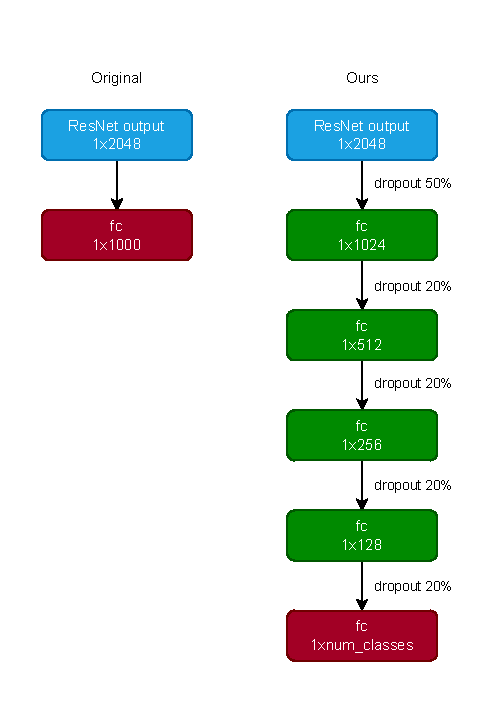
\includegraphics[width=0.5\textwidth]{figures/resnet_funnel.pdf}
      \caption{ResNet-50 architecture with a funnel layer for classification.
            Blue blocks represent the input from the ResNet-50 architecture,
            red blocks represent the final output layer,
            and green blocks represent our new funnel layers.}
      \label{fig:resnet_funnel}
\end{figure}

\subsubsection{Training Procedure}

In our initial training runs,
we observe severe overfitting on the training data as can be seen in Figure~\ref{fig:overfitting}.
To mitigate this, we apply several regularisation techniques:
\begin{itemize}
      \item \textbf{Dropout}~\cite{hinton_improving_2012}:
            As can be seen in Figure~\ref{fig:resnet_funnel},
            our fully connected layers contain dropout layers between them at rates of 0.5 and 0.2.
            Dropout is a regularisation technique that randomly sets a fraction of the input units to zero during training,
            which reinforces the model to learn more robust features and thereby reduces overfitting.
      \item \textbf{Data Augmentation}:
            We apply data augmentation techniques to our training data,
            such as random cropping, horizontal flipping, random erasing, and color jittering.
            These techniques artificially increase the size of our training dataset
            and help the model to generalise better by exposing it to a wider variety of input data.
\end{itemize}

\begin{figure}[ht]
      \centering
      \scalebox{0.6}{%% Creator: Matplotlib, PGF backend
%%
%% To include the figure in your LaTeX document, write
%%   \input{<filename>.pgf}
%%
%% Make sure the required packages are loaded in your preamble
%%   \usepackage{pgf}
%%
%% Also ensure that all the required font packages are loaded; for instance,
%% the lmodern package is sometimes necessary when using math font.
%%   \usepackage{lmodern}
%%
%% Figures using additional raster images can only be included by \input if
%% they are in the same directory as the main LaTeX file. For loading figures
%% from other directories you can use the `import` package
%%   \usepackage{import}
%%
%% and then include the figures with
%%   \import{<path to file>}{<filename>.pgf}
%%
%% Matplotlib used the following preamble
%%   \def\mathdefault#1{#1}
%%   \everymath=\expandafter{\the\everymath\displaystyle}
%%   \IfFileExists{scrextend.sty}{
%%     \usepackage[fontsize=11.000000pt]{scrextend}
%%   }{
%%     \renewcommand{\normalsize}{\fontsize{11.000000}{13.200000}\selectfont}
%%     \normalsize
%%   }
%%   
%%   \ifdefined\pdftexversion\else  % non-pdftex case.
%%     \usepackage{fontspec}
%%     \setmainfont{DejaVuSerif.ttf}[Path=\detokenize{/home/sentinel/.conda/envs/master-thesis/lib/python3.13/site-packages/matplotlib/mpl-data/fonts/ttf/}]
%%     \setsansfont{DejaVuSans.ttf}[Path=\detokenize{/home/sentinel/.conda/envs/master-thesis/lib/python3.13/site-packages/matplotlib/mpl-data/fonts/ttf/}]
%%     \setmonofont{DejaVuSansMono.ttf}[Path=\detokenize{/home/sentinel/.conda/envs/master-thesis/lib/python3.13/site-packages/matplotlib/mpl-data/fonts/ttf/}]
%%   \fi
%%   \makeatletter\@ifpackageloaded{underscore}{}{\usepackage[strings]{underscore}}\makeatother
%%
\begingroup%
\makeatletter%
\begin{pgfpicture}%
\pgfpathrectangle{\pgfpointorigin}{\pgfqpoint{5.344961in}{3.951110in}}%
\pgfusepath{use as bounding box, clip}%
\begin{pgfscope}%
\pgfsetbuttcap%
\pgfsetmiterjoin%
\definecolor{currentfill}{rgb}{1.000000,1.000000,1.000000}%
\pgfsetfillcolor{currentfill}%
\pgfsetlinewidth{0.000000pt}%
\definecolor{currentstroke}{rgb}{1.000000,1.000000,1.000000}%
\pgfsetstrokecolor{currentstroke}%
\pgfsetdash{}{0pt}%
\pgfpathmoveto{\pgfqpoint{0.000000in}{0.000000in}}%
\pgfpathlineto{\pgfqpoint{5.344961in}{0.000000in}}%
\pgfpathlineto{\pgfqpoint{5.344961in}{3.951110in}}%
\pgfpathlineto{\pgfqpoint{0.000000in}{3.951110in}}%
\pgfpathlineto{\pgfqpoint{0.000000in}{0.000000in}}%
\pgfpathclose%
\pgfusepath{fill}%
\end{pgfscope}%
\begin{pgfscope}%
\pgfsetbuttcap%
\pgfsetmiterjoin%
\definecolor{currentfill}{rgb}{1.000000,1.000000,1.000000}%
\pgfsetfillcolor{currentfill}%
\pgfsetlinewidth{0.000000pt}%
\definecolor{currentstroke}{rgb}{0.000000,0.000000,0.000000}%
\pgfsetstrokecolor{currentstroke}%
\pgfsetstrokeopacity{0.000000}%
\pgfsetdash{}{0pt}%
\pgfpathmoveto{\pgfqpoint{0.594961in}{0.548486in}}%
\pgfpathlineto{\pgfqpoint{5.244961in}{0.548486in}}%
\pgfpathlineto{\pgfqpoint{5.244961in}{3.628486in}}%
\pgfpathlineto{\pgfqpoint{0.594961in}{3.628486in}}%
\pgfpathlineto{\pgfqpoint{0.594961in}{0.548486in}}%
\pgfpathclose%
\pgfusepath{fill}%
\end{pgfscope}%
\begin{pgfscope}%
\pgfsetbuttcap%
\pgfsetroundjoin%
\definecolor{currentfill}{rgb}{0.000000,0.000000,0.000000}%
\pgfsetfillcolor{currentfill}%
\pgfsetlinewidth{0.803000pt}%
\definecolor{currentstroke}{rgb}{0.000000,0.000000,0.000000}%
\pgfsetstrokecolor{currentstroke}%
\pgfsetdash{}{0pt}%
\pgfsys@defobject{currentmarker}{\pgfqpoint{0.000000in}{-0.048611in}}{\pgfqpoint{0.000000in}{0.000000in}}{%
\pgfpathmoveto{\pgfqpoint{0.000000in}{0.000000in}}%
\pgfpathlineto{\pgfqpoint{0.000000in}{-0.048611in}}%
\pgfusepath{stroke,fill}%
}%
\begin{pgfscope}%
\pgfsys@transformshift{0.799717in}{0.548486in}%
\pgfsys@useobject{currentmarker}{}%
\end{pgfscope}%
\end{pgfscope}%
\begin{pgfscope}%
\definecolor{textcolor}{rgb}{0.000000,0.000000,0.000000}%
\pgfsetstrokecolor{textcolor}%
\pgfsetfillcolor{textcolor}%
\pgftext[x=0.799717in,y=0.451264in,,top]{\color{textcolor}{\fontsize{11.000000}{13.200000}\selectfont\catcode`\^=\active\def^{\ifmmode\sp\else\^{}\fi}\catcode`\%=\active\def%{\%}$\mathdefault{0}$}}%
\end{pgfscope}%
\begin{pgfscope}%
\pgfsetbuttcap%
\pgfsetroundjoin%
\definecolor{currentfill}{rgb}{0.000000,0.000000,0.000000}%
\pgfsetfillcolor{currentfill}%
\pgfsetlinewidth{0.803000pt}%
\definecolor{currentstroke}{rgb}{0.000000,0.000000,0.000000}%
\pgfsetstrokecolor{currentstroke}%
\pgfsetdash{}{0pt}%
\pgfsys@defobject{currentmarker}{\pgfqpoint{0.000000in}{-0.048611in}}{\pgfqpoint{0.000000in}{0.000000in}}{%
\pgfpathmoveto{\pgfqpoint{0.000000in}{0.000000in}}%
\pgfpathlineto{\pgfqpoint{0.000000in}{-0.048611in}}%
\pgfusepath{stroke,fill}%
}%
\begin{pgfscope}%
\pgfsys@transformshift{1.473924in}{0.548486in}%
\pgfsys@useobject{currentmarker}{}%
\end{pgfscope}%
\end{pgfscope}%
\begin{pgfscope}%
\definecolor{textcolor}{rgb}{0.000000,0.000000,0.000000}%
\pgfsetstrokecolor{textcolor}%
\pgfsetfillcolor{textcolor}%
\pgftext[x=1.473924in,y=0.451264in,,top]{\color{textcolor}{\fontsize{11.000000}{13.200000}\selectfont\catcode`\^=\active\def^{\ifmmode\sp\else\^{}\fi}\catcode`\%=\active\def%{\%}$\mathdefault{5000}$}}%
\end{pgfscope}%
\begin{pgfscope}%
\pgfsetbuttcap%
\pgfsetroundjoin%
\definecolor{currentfill}{rgb}{0.000000,0.000000,0.000000}%
\pgfsetfillcolor{currentfill}%
\pgfsetlinewidth{0.803000pt}%
\definecolor{currentstroke}{rgb}{0.000000,0.000000,0.000000}%
\pgfsetstrokecolor{currentstroke}%
\pgfsetdash{}{0pt}%
\pgfsys@defobject{currentmarker}{\pgfqpoint{0.000000in}{-0.048611in}}{\pgfqpoint{0.000000in}{0.000000in}}{%
\pgfpathmoveto{\pgfqpoint{0.000000in}{0.000000in}}%
\pgfpathlineto{\pgfqpoint{0.000000in}{-0.048611in}}%
\pgfusepath{stroke,fill}%
}%
\begin{pgfscope}%
\pgfsys@transformshift{2.148130in}{0.548486in}%
\pgfsys@useobject{currentmarker}{}%
\end{pgfscope}%
\end{pgfscope}%
\begin{pgfscope}%
\definecolor{textcolor}{rgb}{0.000000,0.000000,0.000000}%
\pgfsetstrokecolor{textcolor}%
\pgfsetfillcolor{textcolor}%
\pgftext[x=2.148130in,y=0.451264in,,top]{\color{textcolor}{\fontsize{11.000000}{13.200000}\selectfont\catcode`\^=\active\def^{\ifmmode\sp\else\^{}\fi}\catcode`\%=\active\def%{\%}$\mathdefault{10000}$}}%
\end{pgfscope}%
\begin{pgfscope}%
\pgfsetbuttcap%
\pgfsetroundjoin%
\definecolor{currentfill}{rgb}{0.000000,0.000000,0.000000}%
\pgfsetfillcolor{currentfill}%
\pgfsetlinewidth{0.803000pt}%
\definecolor{currentstroke}{rgb}{0.000000,0.000000,0.000000}%
\pgfsetstrokecolor{currentstroke}%
\pgfsetdash{}{0pt}%
\pgfsys@defobject{currentmarker}{\pgfqpoint{0.000000in}{-0.048611in}}{\pgfqpoint{0.000000in}{0.000000in}}{%
\pgfpathmoveto{\pgfqpoint{0.000000in}{0.000000in}}%
\pgfpathlineto{\pgfqpoint{0.000000in}{-0.048611in}}%
\pgfusepath{stroke,fill}%
}%
\begin{pgfscope}%
\pgfsys@transformshift{2.822336in}{0.548486in}%
\pgfsys@useobject{currentmarker}{}%
\end{pgfscope}%
\end{pgfscope}%
\begin{pgfscope}%
\definecolor{textcolor}{rgb}{0.000000,0.000000,0.000000}%
\pgfsetstrokecolor{textcolor}%
\pgfsetfillcolor{textcolor}%
\pgftext[x=2.822336in,y=0.451264in,,top]{\color{textcolor}{\fontsize{11.000000}{13.200000}\selectfont\catcode`\^=\active\def^{\ifmmode\sp\else\^{}\fi}\catcode`\%=\active\def%{\%}$\mathdefault{15000}$}}%
\end{pgfscope}%
\begin{pgfscope}%
\pgfsetbuttcap%
\pgfsetroundjoin%
\definecolor{currentfill}{rgb}{0.000000,0.000000,0.000000}%
\pgfsetfillcolor{currentfill}%
\pgfsetlinewidth{0.803000pt}%
\definecolor{currentstroke}{rgb}{0.000000,0.000000,0.000000}%
\pgfsetstrokecolor{currentstroke}%
\pgfsetdash{}{0pt}%
\pgfsys@defobject{currentmarker}{\pgfqpoint{0.000000in}{-0.048611in}}{\pgfqpoint{0.000000in}{0.000000in}}{%
\pgfpathmoveto{\pgfqpoint{0.000000in}{0.000000in}}%
\pgfpathlineto{\pgfqpoint{0.000000in}{-0.048611in}}%
\pgfusepath{stroke,fill}%
}%
\begin{pgfscope}%
\pgfsys@transformshift{3.496542in}{0.548486in}%
\pgfsys@useobject{currentmarker}{}%
\end{pgfscope}%
\end{pgfscope}%
\begin{pgfscope}%
\definecolor{textcolor}{rgb}{0.000000,0.000000,0.000000}%
\pgfsetstrokecolor{textcolor}%
\pgfsetfillcolor{textcolor}%
\pgftext[x=3.496542in,y=0.451264in,,top]{\color{textcolor}{\fontsize{11.000000}{13.200000}\selectfont\catcode`\^=\active\def^{\ifmmode\sp\else\^{}\fi}\catcode`\%=\active\def%{\%}$\mathdefault{20000}$}}%
\end{pgfscope}%
\begin{pgfscope}%
\pgfsetbuttcap%
\pgfsetroundjoin%
\definecolor{currentfill}{rgb}{0.000000,0.000000,0.000000}%
\pgfsetfillcolor{currentfill}%
\pgfsetlinewidth{0.803000pt}%
\definecolor{currentstroke}{rgb}{0.000000,0.000000,0.000000}%
\pgfsetstrokecolor{currentstroke}%
\pgfsetdash{}{0pt}%
\pgfsys@defobject{currentmarker}{\pgfqpoint{0.000000in}{-0.048611in}}{\pgfqpoint{0.000000in}{0.000000in}}{%
\pgfpathmoveto{\pgfqpoint{0.000000in}{0.000000in}}%
\pgfpathlineto{\pgfqpoint{0.000000in}{-0.048611in}}%
\pgfusepath{stroke,fill}%
}%
\begin{pgfscope}%
\pgfsys@transformshift{4.170748in}{0.548486in}%
\pgfsys@useobject{currentmarker}{}%
\end{pgfscope}%
\end{pgfscope}%
\begin{pgfscope}%
\definecolor{textcolor}{rgb}{0.000000,0.000000,0.000000}%
\pgfsetstrokecolor{textcolor}%
\pgfsetfillcolor{textcolor}%
\pgftext[x=4.170748in,y=0.451264in,,top]{\color{textcolor}{\fontsize{11.000000}{13.200000}\selectfont\catcode`\^=\active\def^{\ifmmode\sp\else\^{}\fi}\catcode`\%=\active\def%{\%}$\mathdefault{25000}$}}%
\end{pgfscope}%
\begin{pgfscope}%
\pgfsetbuttcap%
\pgfsetroundjoin%
\definecolor{currentfill}{rgb}{0.000000,0.000000,0.000000}%
\pgfsetfillcolor{currentfill}%
\pgfsetlinewidth{0.803000pt}%
\definecolor{currentstroke}{rgb}{0.000000,0.000000,0.000000}%
\pgfsetstrokecolor{currentstroke}%
\pgfsetdash{}{0pt}%
\pgfsys@defobject{currentmarker}{\pgfqpoint{0.000000in}{-0.048611in}}{\pgfqpoint{0.000000in}{0.000000in}}{%
\pgfpathmoveto{\pgfqpoint{0.000000in}{0.000000in}}%
\pgfpathlineto{\pgfqpoint{0.000000in}{-0.048611in}}%
\pgfusepath{stroke,fill}%
}%
\begin{pgfscope}%
\pgfsys@transformshift{4.844954in}{0.548486in}%
\pgfsys@useobject{currentmarker}{}%
\end{pgfscope}%
\end{pgfscope}%
\begin{pgfscope}%
\definecolor{textcolor}{rgb}{0.000000,0.000000,0.000000}%
\pgfsetstrokecolor{textcolor}%
\pgfsetfillcolor{textcolor}%
\pgftext[x=4.844954in,y=0.451264in,,top]{\color{textcolor}{\fontsize{11.000000}{13.200000}\selectfont\catcode`\^=\active\def^{\ifmmode\sp\else\^{}\fi}\catcode`\%=\active\def%{\%}$\mathdefault{30000}$}}%
\end{pgfscope}%
\begin{pgfscope}%
\definecolor{textcolor}{rgb}{0.000000,0.000000,0.000000}%
\pgfsetstrokecolor{textcolor}%
\pgfsetfillcolor{textcolor}%
\pgftext[x=2.919961in,y=0.247854in,,top]{\color{textcolor}{\fontsize{11.000000}{13.200000}\selectfont\catcode`\^=\active\def^{\ifmmode\sp\else\^{}\fi}\catcode`\%=\active\def%{\%}Steps}}%
\end{pgfscope}%
\begin{pgfscope}%
\pgfsetbuttcap%
\pgfsetroundjoin%
\definecolor{currentfill}{rgb}{0.000000,0.000000,0.000000}%
\pgfsetfillcolor{currentfill}%
\pgfsetlinewidth{0.803000pt}%
\definecolor{currentstroke}{rgb}{0.000000,0.000000,0.000000}%
\pgfsetstrokecolor{currentstroke}%
\pgfsetdash{}{0pt}%
\pgfsys@defobject{currentmarker}{\pgfqpoint{-0.048611in}{0.000000in}}{\pgfqpoint{-0.000000in}{0.000000in}}{%
\pgfpathmoveto{\pgfqpoint{-0.000000in}{0.000000in}}%
\pgfpathlineto{\pgfqpoint{-0.048611in}{0.000000in}}%
\pgfusepath{stroke,fill}%
}%
\begin{pgfscope}%
\pgfsys@transformshift{0.594961in}{0.688486in}%
\pgfsys@useobject{currentmarker}{}%
\end{pgfscope}%
\end{pgfscope}%
\begin{pgfscope}%
\definecolor{textcolor}{rgb}{0.000000,0.000000,0.000000}%
\pgfsetstrokecolor{textcolor}%
\pgfsetfillcolor{textcolor}%
\pgftext[x=0.303410in, y=0.630449in, left, base]{\color{textcolor}{\fontsize{11.000000}{13.200000}\selectfont\catcode`\^=\active\def^{\ifmmode\sp\else\^{}\fi}\catcode`\%=\active\def%{\%}$\mathdefault{0.0}$}}%
\end{pgfscope}%
\begin{pgfscope}%
\pgfsetbuttcap%
\pgfsetroundjoin%
\definecolor{currentfill}{rgb}{0.000000,0.000000,0.000000}%
\pgfsetfillcolor{currentfill}%
\pgfsetlinewidth{0.803000pt}%
\definecolor{currentstroke}{rgb}{0.000000,0.000000,0.000000}%
\pgfsetstrokecolor{currentstroke}%
\pgfsetdash{}{0pt}%
\pgfsys@defobject{currentmarker}{\pgfqpoint{-0.048611in}{0.000000in}}{\pgfqpoint{-0.000000in}{0.000000in}}{%
\pgfpathmoveto{\pgfqpoint{-0.000000in}{0.000000in}}%
\pgfpathlineto{\pgfqpoint{-0.048611in}{0.000000in}}%
\pgfusepath{stroke,fill}%
}%
\begin{pgfscope}%
\pgfsys@transformshift{0.594961in}{1.248486in}%
\pgfsys@useobject{currentmarker}{}%
\end{pgfscope}%
\end{pgfscope}%
\begin{pgfscope}%
\definecolor{textcolor}{rgb}{0.000000,0.000000,0.000000}%
\pgfsetstrokecolor{textcolor}%
\pgfsetfillcolor{textcolor}%
\pgftext[x=0.303410in, y=1.190449in, left, base]{\color{textcolor}{\fontsize{11.000000}{13.200000}\selectfont\catcode`\^=\active\def^{\ifmmode\sp\else\^{}\fi}\catcode`\%=\active\def%{\%}$\mathdefault{0.2}$}}%
\end{pgfscope}%
\begin{pgfscope}%
\pgfsetbuttcap%
\pgfsetroundjoin%
\definecolor{currentfill}{rgb}{0.000000,0.000000,0.000000}%
\pgfsetfillcolor{currentfill}%
\pgfsetlinewidth{0.803000pt}%
\definecolor{currentstroke}{rgb}{0.000000,0.000000,0.000000}%
\pgfsetstrokecolor{currentstroke}%
\pgfsetdash{}{0pt}%
\pgfsys@defobject{currentmarker}{\pgfqpoint{-0.048611in}{0.000000in}}{\pgfqpoint{-0.000000in}{0.000000in}}{%
\pgfpathmoveto{\pgfqpoint{-0.000000in}{0.000000in}}%
\pgfpathlineto{\pgfqpoint{-0.048611in}{0.000000in}}%
\pgfusepath{stroke,fill}%
}%
\begin{pgfscope}%
\pgfsys@transformshift{0.594961in}{1.808486in}%
\pgfsys@useobject{currentmarker}{}%
\end{pgfscope}%
\end{pgfscope}%
\begin{pgfscope}%
\definecolor{textcolor}{rgb}{0.000000,0.000000,0.000000}%
\pgfsetstrokecolor{textcolor}%
\pgfsetfillcolor{textcolor}%
\pgftext[x=0.303410in, y=1.750449in, left, base]{\color{textcolor}{\fontsize{11.000000}{13.200000}\selectfont\catcode`\^=\active\def^{\ifmmode\sp\else\^{}\fi}\catcode`\%=\active\def%{\%}$\mathdefault{0.4}$}}%
\end{pgfscope}%
\begin{pgfscope}%
\pgfsetbuttcap%
\pgfsetroundjoin%
\definecolor{currentfill}{rgb}{0.000000,0.000000,0.000000}%
\pgfsetfillcolor{currentfill}%
\pgfsetlinewidth{0.803000pt}%
\definecolor{currentstroke}{rgb}{0.000000,0.000000,0.000000}%
\pgfsetstrokecolor{currentstroke}%
\pgfsetdash{}{0pt}%
\pgfsys@defobject{currentmarker}{\pgfqpoint{-0.048611in}{0.000000in}}{\pgfqpoint{-0.000000in}{0.000000in}}{%
\pgfpathmoveto{\pgfqpoint{-0.000000in}{0.000000in}}%
\pgfpathlineto{\pgfqpoint{-0.048611in}{0.000000in}}%
\pgfusepath{stroke,fill}%
}%
\begin{pgfscope}%
\pgfsys@transformshift{0.594961in}{2.368486in}%
\pgfsys@useobject{currentmarker}{}%
\end{pgfscope}%
\end{pgfscope}%
\begin{pgfscope}%
\definecolor{textcolor}{rgb}{0.000000,0.000000,0.000000}%
\pgfsetstrokecolor{textcolor}%
\pgfsetfillcolor{textcolor}%
\pgftext[x=0.303410in, y=2.310449in, left, base]{\color{textcolor}{\fontsize{11.000000}{13.200000}\selectfont\catcode`\^=\active\def^{\ifmmode\sp\else\^{}\fi}\catcode`\%=\active\def%{\%}$\mathdefault{0.6}$}}%
\end{pgfscope}%
\begin{pgfscope}%
\pgfsetbuttcap%
\pgfsetroundjoin%
\definecolor{currentfill}{rgb}{0.000000,0.000000,0.000000}%
\pgfsetfillcolor{currentfill}%
\pgfsetlinewidth{0.803000pt}%
\definecolor{currentstroke}{rgb}{0.000000,0.000000,0.000000}%
\pgfsetstrokecolor{currentstroke}%
\pgfsetdash{}{0pt}%
\pgfsys@defobject{currentmarker}{\pgfqpoint{-0.048611in}{0.000000in}}{\pgfqpoint{-0.000000in}{0.000000in}}{%
\pgfpathmoveto{\pgfqpoint{-0.000000in}{0.000000in}}%
\pgfpathlineto{\pgfqpoint{-0.048611in}{0.000000in}}%
\pgfusepath{stroke,fill}%
}%
\begin{pgfscope}%
\pgfsys@transformshift{0.594961in}{2.928486in}%
\pgfsys@useobject{currentmarker}{}%
\end{pgfscope}%
\end{pgfscope}%
\begin{pgfscope}%
\definecolor{textcolor}{rgb}{0.000000,0.000000,0.000000}%
\pgfsetstrokecolor{textcolor}%
\pgfsetfillcolor{textcolor}%
\pgftext[x=0.303410in, y=2.870449in, left, base]{\color{textcolor}{\fontsize{11.000000}{13.200000}\selectfont\catcode`\^=\active\def^{\ifmmode\sp\else\^{}\fi}\catcode`\%=\active\def%{\%}$\mathdefault{0.8}$}}%
\end{pgfscope}%
\begin{pgfscope}%
\pgfsetbuttcap%
\pgfsetroundjoin%
\definecolor{currentfill}{rgb}{0.000000,0.000000,0.000000}%
\pgfsetfillcolor{currentfill}%
\pgfsetlinewidth{0.803000pt}%
\definecolor{currentstroke}{rgb}{0.000000,0.000000,0.000000}%
\pgfsetstrokecolor{currentstroke}%
\pgfsetdash{}{0pt}%
\pgfsys@defobject{currentmarker}{\pgfqpoint{-0.048611in}{0.000000in}}{\pgfqpoint{-0.000000in}{0.000000in}}{%
\pgfpathmoveto{\pgfqpoint{-0.000000in}{0.000000in}}%
\pgfpathlineto{\pgfqpoint{-0.048611in}{0.000000in}}%
\pgfusepath{stroke,fill}%
}%
\begin{pgfscope}%
\pgfsys@transformshift{0.594961in}{3.488486in}%
\pgfsys@useobject{currentmarker}{}%
\end{pgfscope}%
\end{pgfscope}%
\begin{pgfscope}%
\definecolor{textcolor}{rgb}{0.000000,0.000000,0.000000}%
\pgfsetstrokecolor{textcolor}%
\pgfsetfillcolor{textcolor}%
\pgftext[x=0.303410in, y=3.430449in, left, base]{\color{textcolor}{\fontsize{11.000000}{13.200000}\selectfont\catcode`\^=\active\def^{\ifmmode\sp\else\^{}\fi}\catcode`\%=\active\def%{\%}$\mathdefault{1.0}$}}%
\end{pgfscope}%
\begin{pgfscope}%
\definecolor{textcolor}{rgb}{0.000000,0.000000,0.000000}%
\pgfsetstrokecolor{textcolor}%
\pgfsetfillcolor{textcolor}%
\pgftext[x=0.247854in,y=2.088486in,,bottom,rotate=90.000000]{\color{textcolor}{\fontsize{11.000000}{13.200000}\selectfont\catcode`\^=\active\def^{\ifmmode\sp\else\^{}\fi}\catcode`\%=\active\def%{\%}Accuracy}}%
\end{pgfscope}%
\begin{pgfscope}%
\pgfpathrectangle{\pgfqpoint{0.594961in}{0.548486in}}{\pgfqpoint{4.650000in}{3.080000in}}%
\pgfusepath{clip}%
\pgfsetrectcap%
\pgfsetroundjoin%
\pgfsetlinewidth{1.505625pt}%
\definecolor{currentstroke}{rgb}{0.121569,0.466667,0.705882}%
\pgfsetstrokecolor{currentstroke}%
\pgfsetdash{}{0pt}%
\pgfpathmoveto{\pgfqpoint{0.806325in}{0.688486in}}%
\pgfpathlineto{\pgfqpoint{0.813067in}{0.754111in}}%
\pgfpathlineto{\pgfqpoint{0.819809in}{0.732236in}}%
\pgfpathlineto{\pgfqpoint{0.826551in}{0.765049in}}%
\pgfpathlineto{\pgfqpoint{0.833293in}{0.699424in}}%
\pgfpathlineto{\pgfqpoint{0.840035in}{0.721299in}}%
\pgfpathlineto{\pgfqpoint{0.846777in}{0.721299in}}%
\pgfpathlineto{\pgfqpoint{0.853519in}{0.699424in}}%
\pgfpathlineto{\pgfqpoint{0.860261in}{0.754111in}}%
\pgfpathlineto{\pgfqpoint{0.867003in}{0.721299in}}%
\pgfpathlineto{\pgfqpoint{0.873745in}{0.754111in}}%
\pgfpathlineto{\pgfqpoint{0.880487in}{0.743174in}}%
\pgfpathlineto{\pgfqpoint{0.887229in}{0.830674in}}%
\pgfpathlineto{\pgfqpoint{0.893971in}{0.797861in}}%
\pgfpathlineto{\pgfqpoint{0.900713in}{0.775986in}}%
\pgfpathlineto{\pgfqpoint{0.907456in}{0.797861in}}%
\pgfpathlineto{\pgfqpoint{0.914198in}{0.841611in}}%
\pgfpathlineto{\pgfqpoint{0.920940in}{0.819736in}}%
\pgfpathlineto{\pgfqpoint{0.927682in}{0.819736in}}%
\pgfpathlineto{\pgfqpoint{0.934424in}{0.885361in}}%
\pgfpathlineto{\pgfqpoint{0.941166in}{0.808799in}}%
\pgfpathlineto{\pgfqpoint{0.947908in}{0.797861in}}%
\pgfpathlineto{\pgfqpoint{0.954650in}{0.819736in}}%
\pgfpathlineto{\pgfqpoint{0.968134in}{0.797861in}}%
\pgfpathlineto{\pgfqpoint{0.974876in}{0.797861in}}%
\pgfpathlineto{\pgfqpoint{0.981618in}{0.852549in}}%
\pgfpathlineto{\pgfqpoint{0.988360in}{0.808799in}}%
\pgfpathlineto{\pgfqpoint{0.995102in}{0.863486in}}%
\pgfpathlineto{\pgfqpoint{1.001844in}{0.841611in}}%
\pgfpathlineto{\pgfqpoint{1.008586in}{0.940049in}}%
\pgfpathlineto{\pgfqpoint{1.015329in}{0.940049in}}%
\pgfpathlineto{\pgfqpoint{1.022071in}{1.016611in}}%
\pgfpathlineto{\pgfqpoint{1.028813in}{0.961924in}}%
\pgfpathlineto{\pgfqpoint{1.035555in}{0.950986in}}%
\pgfpathlineto{\pgfqpoint{1.042297in}{0.994736in}}%
\pgfpathlineto{\pgfqpoint{1.049039in}{0.940049in}}%
\pgfpathlineto{\pgfqpoint{1.055781in}{1.049424in}}%
\pgfpathlineto{\pgfqpoint{1.062523in}{1.060361in}}%
\pgfpathlineto{\pgfqpoint{1.069265in}{1.104111in}}%
\pgfpathlineto{\pgfqpoint{1.076007in}{0.950986in}}%
\pgfpathlineto{\pgfqpoint{1.082749in}{1.016611in}}%
\pgfpathlineto{\pgfqpoint{1.089491in}{1.071299in}}%
\pgfpathlineto{\pgfqpoint{1.096233in}{1.093174in}}%
\pgfpathlineto{\pgfqpoint{1.102975in}{1.180674in}}%
\pgfpathlineto{\pgfqpoint{1.109717in}{1.060361in}}%
\pgfpathlineto{\pgfqpoint{1.116459in}{1.136924in}}%
\pgfpathlineto{\pgfqpoint{1.129944in}{1.093174in}}%
\pgfpathlineto{\pgfqpoint{1.136686in}{1.093174in}}%
\pgfpathlineto{\pgfqpoint{1.143428in}{1.027549in}}%
\pgfpathlineto{\pgfqpoint{1.150170in}{1.136924in}}%
\pgfpathlineto{\pgfqpoint{1.156912in}{0.841611in}}%
\pgfpathlineto{\pgfqpoint{1.163654in}{1.125986in}}%
\pgfpathlineto{\pgfqpoint{1.170396in}{1.071299in}}%
\pgfpathlineto{\pgfqpoint{1.177138in}{1.213486in}}%
\pgfpathlineto{\pgfqpoint{1.183880in}{1.202549in}}%
\pgfpathlineto{\pgfqpoint{1.190622in}{1.300986in}}%
\pgfpathlineto{\pgfqpoint{1.197364in}{1.213486in}}%
\pgfpathlineto{\pgfqpoint{1.204106in}{1.224424in}}%
\pgfpathlineto{\pgfqpoint{1.210848in}{1.344736in}}%
\pgfpathlineto{\pgfqpoint{1.217590in}{1.377549in}}%
\pgfpathlineto{\pgfqpoint{1.224332in}{1.333799in}}%
\pgfpathlineto{\pgfqpoint{1.231074in}{1.443174in}}%
\pgfpathlineto{\pgfqpoint{1.237817in}{1.377549in}}%
\pgfpathlineto{\pgfqpoint{1.244559in}{1.355674in}}%
\pgfpathlineto{\pgfqpoint{1.251301in}{1.410361in}}%
\pgfpathlineto{\pgfqpoint{1.258043in}{1.388486in}}%
\pgfpathlineto{\pgfqpoint{1.264785in}{1.410361in}}%
\pgfpathlineto{\pgfqpoint{1.271527in}{1.486924in}}%
\pgfpathlineto{\pgfqpoint{1.278269in}{1.443174in}}%
\pgfpathlineto{\pgfqpoint{1.285011in}{1.574424in}}%
\pgfpathlineto{\pgfqpoint{1.291753in}{1.519736in}}%
\pgfpathlineto{\pgfqpoint{1.298495in}{1.629111in}}%
\pgfpathlineto{\pgfqpoint{1.305237in}{1.497861in}}%
\pgfpathlineto{\pgfqpoint{1.311979in}{1.618174in}}%
\pgfpathlineto{\pgfqpoint{1.318721in}{1.661924in}}%
\pgfpathlineto{\pgfqpoint{1.325463in}{1.475986in}}%
\pgfpathlineto{\pgfqpoint{1.332205in}{1.661924in}}%
\pgfpathlineto{\pgfqpoint{1.338947in}{1.530674in}}%
\pgfpathlineto{\pgfqpoint{1.345690in}{1.596299in}}%
\pgfpathlineto{\pgfqpoint{1.352432in}{1.574424in}}%
\pgfpathlineto{\pgfqpoint{1.359174in}{1.607236in}}%
\pgfpathlineto{\pgfqpoint{1.365916in}{1.705674in}}%
\pgfpathlineto{\pgfqpoint{1.372658in}{1.782236in}}%
\pgfpathlineto{\pgfqpoint{1.379400in}{1.541611in}}%
\pgfpathlineto{\pgfqpoint{1.392884in}{1.716611in}}%
\pgfpathlineto{\pgfqpoint{1.399626in}{1.771299in}}%
\pgfpathlineto{\pgfqpoint{1.406368in}{1.738486in}}%
\pgfpathlineto{\pgfqpoint{1.413110in}{1.596299in}}%
\pgfpathlineto{\pgfqpoint{1.419852in}{1.650986in}}%
\pgfpathlineto{\pgfqpoint{1.426594in}{1.880674in}}%
\pgfpathlineto{\pgfqpoint{1.433336in}{1.771299in}}%
\pgfpathlineto{\pgfqpoint{1.440078in}{1.858799in}}%
\pgfpathlineto{\pgfqpoint{1.446820in}{1.596299in}}%
\pgfpathlineto{\pgfqpoint{1.453563in}{1.705674in}}%
\pgfpathlineto{\pgfqpoint{1.467047in}{1.640049in}}%
\pgfpathlineto{\pgfqpoint{1.473789in}{1.902549in}}%
\pgfpathlineto{\pgfqpoint{1.480531in}{2.088486in}}%
\pgfpathlineto{\pgfqpoint{1.487273in}{1.869736in}}%
\pgfpathlineto{\pgfqpoint{1.494015in}{1.869736in}}%
\pgfpathlineto{\pgfqpoint{1.500757in}{1.847861in}}%
\pgfpathlineto{\pgfqpoint{1.507499in}{1.836924in}}%
\pgfpathlineto{\pgfqpoint{1.514241in}{2.077549in}}%
\pgfpathlineto{\pgfqpoint{1.520983in}{1.869736in}}%
\pgfpathlineto{\pgfqpoint{1.527725in}{1.979111in}}%
\pgfpathlineto{\pgfqpoint{1.534467in}{2.000986in}}%
\pgfpathlineto{\pgfqpoint{1.541209in}{2.044736in}}%
\pgfpathlineto{\pgfqpoint{1.547951in}{1.858799in}}%
\pgfpathlineto{\pgfqpoint{1.554693in}{1.891611in}}%
\pgfpathlineto{\pgfqpoint{1.561436in}{2.077549in}}%
\pgfpathlineto{\pgfqpoint{1.568178in}{1.990049in}}%
\pgfpathlineto{\pgfqpoint{1.574920in}{1.836924in}}%
\pgfpathlineto{\pgfqpoint{1.581662in}{1.541611in}}%
\pgfpathlineto{\pgfqpoint{1.588404in}{1.935361in}}%
\pgfpathlineto{\pgfqpoint{1.595146in}{1.946299in}}%
\pgfpathlineto{\pgfqpoint{1.601888in}{2.066611in}}%
\pgfpathlineto{\pgfqpoint{1.608630in}{1.935361in}}%
\pgfpathlineto{\pgfqpoint{1.615372in}{1.902549in}}%
\pgfpathlineto{\pgfqpoint{1.622114in}{2.219736in}}%
\pgfpathlineto{\pgfqpoint{1.628856in}{2.055674in}}%
\pgfpathlineto{\pgfqpoint{1.635598in}{2.066611in}}%
\pgfpathlineto{\pgfqpoint{1.642340in}{2.099424in}}%
\pgfpathlineto{\pgfqpoint{1.649082in}{2.263486in}}%
\pgfpathlineto{\pgfqpoint{1.655824in}{2.110361in}}%
\pgfpathlineto{\pgfqpoint{1.662566in}{2.044736in}}%
\pgfpathlineto{\pgfqpoint{1.669309in}{2.175986in}}%
\pgfpathlineto{\pgfqpoint{1.676051in}{2.186924in}}%
\pgfpathlineto{\pgfqpoint{1.682793in}{2.186924in}}%
\pgfpathlineto{\pgfqpoint{1.689535in}{2.252549in}}%
\pgfpathlineto{\pgfqpoint{1.696277in}{2.132236in}}%
\pgfpathlineto{\pgfqpoint{1.703019in}{2.241611in}}%
\pgfpathlineto{\pgfqpoint{1.709761in}{2.022861in}}%
\pgfpathlineto{\pgfqpoint{1.716503in}{2.197861in}}%
\pgfpathlineto{\pgfqpoint{1.723245in}{2.099424in}}%
\pgfpathlineto{\pgfqpoint{1.729987in}{2.252549in}}%
\pgfpathlineto{\pgfqpoint{1.736729in}{2.121299in}}%
\pgfpathlineto{\pgfqpoint{1.743471in}{2.296299in}}%
\pgfpathlineto{\pgfqpoint{1.750213in}{2.165049in}}%
\pgfpathlineto{\pgfqpoint{1.763697in}{2.252549in}}%
\pgfpathlineto{\pgfqpoint{1.770439in}{2.219736in}}%
\pgfpathlineto{\pgfqpoint{1.777182in}{2.416611in}}%
\pgfpathlineto{\pgfqpoint{1.783924in}{2.208799in}}%
\pgfpathlineto{\pgfqpoint{1.790666in}{2.427549in}}%
\pgfpathlineto{\pgfqpoint{1.797408in}{2.296299in}}%
\pgfpathlineto{\pgfqpoint{1.804150in}{2.536924in}}%
\pgfpathlineto{\pgfqpoint{1.810892in}{2.383799in}}%
\pgfpathlineto{\pgfqpoint{1.817634in}{2.416611in}}%
\pgfpathlineto{\pgfqpoint{1.824376in}{2.219736in}}%
\pgfpathlineto{\pgfqpoint{1.831118in}{2.252549in}}%
\pgfpathlineto{\pgfqpoint{1.837860in}{2.329111in}}%
\pgfpathlineto{\pgfqpoint{1.844602in}{2.318174in}}%
\pgfpathlineto{\pgfqpoint{1.851344in}{2.536924in}}%
\pgfpathlineto{\pgfqpoint{1.858086in}{3.138486in}}%
\pgfpathlineto{\pgfqpoint{1.864828in}{2.394736in}}%
\pgfpathlineto{\pgfqpoint{1.871570in}{2.679111in}}%
\pgfpathlineto{\pgfqpoint{1.878312in}{2.613486in}}%
\pgfpathlineto{\pgfqpoint{1.885054in}{2.558799in}}%
\pgfpathlineto{\pgfqpoint{1.891797in}{2.449424in}}%
\pgfpathlineto{\pgfqpoint{1.898539in}{2.438486in}}%
\pgfpathlineto{\pgfqpoint{1.905281in}{2.624424in}}%
\pgfpathlineto{\pgfqpoint{1.912023in}{2.427549in}}%
\pgfpathlineto{\pgfqpoint{1.918765in}{2.493174in}}%
\pgfpathlineto{\pgfqpoint{1.925507in}{2.427549in}}%
\pgfpathlineto{\pgfqpoint{1.932249in}{2.449424in}}%
\pgfpathlineto{\pgfqpoint{1.938991in}{2.580674in}}%
\pgfpathlineto{\pgfqpoint{1.945733in}{2.536924in}}%
\pgfpathlineto{\pgfqpoint{1.952475in}{2.482236in}}%
\pgfpathlineto{\pgfqpoint{1.959217in}{2.493174in}}%
\pgfpathlineto{\pgfqpoint{1.965959in}{2.405674in}}%
\pgfpathlineto{\pgfqpoint{1.972701in}{2.504111in}}%
\pgfpathlineto{\pgfqpoint{1.979443in}{2.525986in}}%
\pgfpathlineto{\pgfqpoint{1.986185in}{2.525986in}}%
\pgfpathlineto{\pgfqpoint{1.992927in}{2.493174in}}%
\pgfpathlineto{\pgfqpoint{1.999670in}{2.613486in}}%
\pgfpathlineto{\pgfqpoint{2.006412in}{2.471299in}}%
\pgfpathlineto{\pgfqpoint{2.013154in}{2.515049in}}%
\pgfpathlineto{\pgfqpoint{2.019896in}{2.471299in}}%
\pgfpathlineto{\pgfqpoint{2.026638in}{2.624424in}}%
\pgfpathlineto{\pgfqpoint{2.033380in}{2.350986in}}%
\pgfpathlineto{\pgfqpoint{2.040122in}{2.525986in}}%
\pgfpathlineto{\pgfqpoint{2.046864in}{2.536924in}}%
\pgfpathlineto{\pgfqpoint{2.053606in}{2.635361in}}%
\pgfpathlineto{\pgfqpoint{2.060348in}{2.536924in}}%
\pgfpathlineto{\pgfqpoint{2.067090in}{2.602549in}}%
\pgfpathlineto{\pgfqpoint{2.073832in}{2.646299in}}%
\pgfpathlineto{\pgfqpoint{2.080574in}{2.952549in}}%
\pgfpathlineto{\pgfqpoint{2.087316in}{3.204111in}}%
\pgfpathlineto{\pgfqpoint{2.094058in}{3.061924in}}%
\pgfpathlineto{\pgfqpoint{2.100800in}{3.061924in}}%
\pgfpathlineto{\pgfqpoint{2.107543in}{3.204111in}}%
\pgfpathlineto{\pgfqpoint{2.114285in}{3.138486in}}%
\pgfpathlineto{\pgfqpoint{2.121027in}{3.225986in}}%
\pgfpathlineto{\pgfqpoint{2.127769in}{3.149424in}}%
\pgfpathlineto{\pgfqpoint{2.134511in}{3.204111in}}%
\pgfpathlineto{\pgfqpoint{2.141253in}{3.204111in}}%
\pgfpathlineto{\pgfqpoint{2.147995in}{3.225986in}}%
\pgfpathlineto{\pgfqpoint{2.154737in}{3.302549in}}%
\pgfpathlineto{\pgfqpoint{2.161479in}{3.269736in}}%
\pgfpathlineto{\pgfqpoint{2.168221in}{3.269736in}}%
\pgfpathlineto{\pgfqpoint{2.174963in}{3.236924in}}%
\pgfpathlineto{\pgfqpoint{2.181705in}{3.357236in}}%
\pgfpathlineto{\pgfqpoint{2.188447in}{3.335361in}}%
\pgfpathlineto{\pgfqpoint{2.195189in}{3.411924in}}%
\pgfpathlineto{\pgfqpoint{2.201931in}{3.390049in}}%
\pgfpathlineto{\pgfqpoint{2.208673in}{3.324424in}}%
\pgfpathlineto{\pgfqpoint{2.215416in}{3.400986in}}%
\pgfpathlineto{\pgfqpoint{2.222158in}{3.346299in}}%
\pgfpathlineto{\pgfqpoint{2.228900in}{3.400986in}}%
\pgfpathlineto{\pgfqpoint{2.235642in}{3.357236in}}%
\pgfpathlineto{\pgfqpoint{2.249126in}{3.291611in}}%
\pgfpathlineto{\pgfqpoint{2.255868in}{3.390049in}}%
\pgfpathlineto{\pgfqpoint{2.262610in}{3.357236in}}%
\pgfpathlineto{\pgfqpoint{2.269352in}{3.390049in}}%
\pgfpathlineto{\pgfqpoint{2.276094in}{3.346299in}}%
\pgfpathlineto{\pgfqpoint{2.282836in}{3.400986in}}%
\pgfpathlineto{\pgfqpoint{2.289578in}{3.357236in}}%
\pgfpathlineto{\pgfqpoint{2.296320in}{3.422861in}}%
\pgfpathlineto{\pgfqpoint{2.303062in}{3.379111in}}%
\pgfpathlineto{\pgfqpoint{2.309804in}{3.422861in}}%
\pgfpathlineto{\pgfqpoint{2.316546in}{3.313486in}}%
\pgfpathlineto{\pgfqpoint{2.323289in}{3.357236in}}%
\pgfpathlineto{\pgfqpoint{2.330031in}{3.357236in}}%
\pgfpathlineto{\pgfqpoint{2.336773in}{3.455674in}}%
\pgfpathlineto{\pgfqpoint{2.343515in}{3.335361in}}%
\pgfpathlineto{\pgfqpoint{2.350257in}{3.422861in}}%
\pgfpathlineto{\pgfqpoint{2.356999in}{3.357236in}}%
\pgfpathlineto{\pgfqpoint{2.363741in}{3.422861in}}%
\pgfpathlineto{\pgfqpoint{2.370483in}{3.411924in}}%
\pgfpathlineto{\pgfqpoint{2.377225in}{3.368174in}}%
\pgfpathlineto{\pgfqpoint{2.383967in}{3.346299in}}%
\pgfpathlineto{\pgfqpoint{2.390709in}{3.411924in}}%
\pgfpathlineto{\pgfqpoint{2.397451in}{3.379111in}}%
\pgfpathlineto{\pgfqpoint{2.404193in}{3.390049in}}%
\pgfpathlineto{\pgfqpoint{2.417677in}{3.433799in}}%
\pgfpathlineto{\pgfqpoint{2.424419in}{3.400986in}}%
\pgfpathlineto{\pgfqpoint{2.431161in}{3.379111in}}%
\pgfpathlineto{\pgfqpoint{2.437904in}{3.346299in}}%
\pgfpathlineto{\pgfqpoint{2.444646in}{3.411924in}}%
\pgfpathlineto{\pgfqpoint{2.458130in}{3.368174in}}%
\pgfpathlineto{\pgfqpoint{2.464872in}{3.422861in}}%
\pgfpathlineto{\pgfqpoint{2.471614in}{3.390049in}}%
\pgfpathlineto{\pgfqpoint{2.478356in}{3.324424in}}%
\pgfpathlineto{\pgfqpoint{2.485098in}{3.422861in}}%
\pgfpathlineto{\pgfqpoint{2.491840in}{3.368174in}}%
\pgfpathlineto{\pgfqpoint{2.498582in}{3.411924in}}%
\pgfpathlineto{\pgfqpoint{2.505324in}{3.390049in}}%
\pgfpathlineto{\pgfqpoint{2.512066in}{3.335361in}}%
\pgfpathlineto{\pgfqpoint{2.518808in}{3.379111in}}%
\pgfpathlineto{\pgfqpoint{2.525550in}{3.411924in}}%
\pgfpathlineto{\pgfqpoint{2.532292in}{3.346299in}}%
\pgfpathlineto{\pgfqpoint{2.539034in}{3.390049in}}%
\pgfpathlineto{\pgfqpoint{2.545777in}{3.346299in}}%
\pgfpathlineto{\pgfqpoint{2.552519in}{3.324424in}}%
\pgfpathlineto{\pgfqpoint{2.559261in}{3.390049in}}%
\pgfpathlineto{\pgfqpoint{2.566003in}{3.357236in}}%
\pgfpathlineto{\pgfqpoint{2.572745in}{3.433799in}}%
\pgfpathlineto{\pgfqpoint{2.579487in}{3.357236in}}%
\pgfpathlineto{\pgfqpoint{2.586229in}{3.357236in}}%
\pgfpathlineto{\pgfqpoint{2.592971in}{3.368174in}}%
\pgfpathlineto{\pgfqpoint{2.599713in}{3.422861in}}%
\pgfpathlineto{\pgfqpoint{2.606455in}{3.433799in}}%
\pgfpathlineto{\pgfqpoint{2.619939in}{3.411924in}}%
\pgfpathlineto{\pgfqpoint{2.626681in}{3.368174in}}%
\pgfpathlineto{\pgfqpoint{2.633423in}{3.400986in}}%
\pgfpathlineto{\pgfqpoint{2.640165in}{3.335361in}}%
\pgfpathlineto{\pgfqpoint{2.646907in}{3.390049in}}%
\pgfpathlineto{\pgfqpoint{2.653650in}{3.422861in}}%
\pgfpathlineto{\pgfqpoint{2.660392in}{3.302549in}}%
\pgfpathlineto{\pgfqpoint{2.667134in}{3.335361in}}%
\pgfpathlineto{\pgfqpoint{2.673876in}{3.335361in}}%
\pgfpathlineto{\pgfqpoint{2.680618in}{3.357236in}}%
\pgfpathlineto{\pgfqpoint{2.687360in}{3.335361in}}%
\pgfpathlineto{\pgfqpoint{2.694102in}{3.422861in}}%
\pgfpathlineto{\pgfqpoint{2.700844in}{3.335361in}}%
\pgfpathlineto{\pgfqpoint{2.707586in}{3.357236in}}%
\pgfpathlineto{\pgfqpoint{2.714328in}{3.400986in}}%
\pgfpathlineto{\pgfqpoint{2.721070in}{3.422861in}}%
\pgfpathlineto{\pgfqpoint{2.727812in}{3.411924in}}%
\pgfpathlineto{\pgfqpoint{2.734554in}{3.346299in}}%
\pgfpathlineto{\pgfqpoint{2.741296in}{3.368174in}}%
\pgfpathlineto{\pgfqpoint{2.748038in}{3.346299in}}%
\pgfpathlineto{\pgfqpoint{2.754780in}{3.357236in}}%
\pgfpathlineto{\pgfqpoint{2.761523in}{3.335361in}}%
\pgfpathlineto{\pgfqpoint{2.768265in}{3.379111in}}%
\pgfpathlineto{\pgfqpoint{2.775007in}{3.291611in}}%
\pgfpathlineto{\pgfqpoint{2.781749in}{3.324424in}}%
\pgfpathlineto{\pgfqpoint{2.788491in}{3.313486in}}%
\pgfpathlineto{\pgfqpoint{2.795233in}{3.379111in}}%
\pgfpathlineto{\pgfqpoint{2.801975in}{3.357236in}}%
\pgfpathlineto{\pgfqpoint{2.808717in}{3.269736in}}%
\pgfpathlineto{\pgfqpoint{2.815459in}{3.346299in}}%
\pgfpathlineto{\pgfqpoint{2.822201in}{3.324424in}}%
\pgfpathlineto{\pgfqpoint{2.828943in}{3.324424in}}%
\pgfpathlineto{\pgfqpoint{2.835685in}{3.422861in}}%
\pgfpathlineto{\pgfqpoint{2.842427in}{3.269736in}}%
\pgfpathlineto{\pgfqpoint{2.849169in}{3.368174in}}%
\pgfpathlineto{\pgfqpoint{2.855911in}{3.335361in}}%
\pgfpathlineto{\pgfqpoint{2.862653in}{3.335361in}}%
\pgfpathlineto{\pgfqpoint{2.876138in}{3.379111in}}%
\pgfpathlineto{\pgfqpoint{2.882880in}{3.357236in}}%
\pgfpathlineto{\pgfqpoint{2.889622in}{3.346299in}}%
\pgfpathlineto{\pgfqpoint{2.896364in}{3.313486in}}%
\pgfpathlineto{\pgfqpoint{2.909848in}{3.313486in}}%
\pgfpathlineto{\pgfqpoint{2.916590in}{3.488486in}}%
\pgfpathlineto{\pgfqpoint{2.923332in}{3.302549in}}%
\pgfpathlineto{\pgfqpoint{2.930074in}{3.379111in}}%
\pgfpathlineto{\pgfqpoint{2.936816in}{3.357236in}}%
\pgfpathlineto{\pgfqpoint{2.943558in}{3.368174in}}%
\pgfpathlineto{\pgfqpoint{2.950300in}{3.400986in}}%
\pgfpathlineto{\pgfqpoint{2.957042in}{3.357236in}}%
\pgfpathlineto{\pgfqpoint{2.970526in}{3.313486in}}%
\pgfpathlineto{\pgfqpoint{2.977268in}{3.379111in}}%
\pgfpathlineto{\pgfqpoint{2.984011in}{3.379111in}}%
\pgfpathlineto{\pgfqpoint{2.990753in}{3.346299in}}%
\pgfpathlineto{\pgfqpoint{2.997495in}{3.368174in}}%
\pgfpathlineto{\pgfqpoint{3.004237in}{3.379111in}}%
\pgfpathlineto{\pgfqpoint{3.010979in}{3.400986in}}%
\pgfpathlineto{\pgfqpoint{3.024463in}{3.335361in}}%
\pgfpathlineto{\pgfqpoint{3.031205in}{3.324424in}}%
\pgfpathlineto{\pgfqpoint{3.037947in}{3.346299in}}%
\pgfpathlineto{\pgfqpoint{3.044689in}{3.357236in}}%
\pgfpathlineto{\pgfqpoint{3.051431in}{3.324424in}}%
\pgfpathlineto{\pgfqpoint{3.058173in}{3.390049in}}%
\pgfpathlineto{\pgfqpoint{3.064915in}{3.346299in}}%
\pgfpathlineto{\pgfqpoint{3.071657in}{3.291611in}}%
\pgfpathlineto{\pgfqpoint{3.078399in}{3.357236in}}%
\pgfpathlineto{\pgfqpoint{3.085141in}{3.400986in}}%
\pgfpathlineto{\pgfqpoint{3.091884in}{3.258799in}}%
\pgfpathlineto{\pgfqpoint{3.105368in}{3.444736in}}%
\pgfpathlineto{\pgfqpoint{3.112110in}{3.368174in}}%
\pgfpathlineto{\pgfqpoint{3.118852in}{3.313486in}}%
\pgfpathlineto{\pgfqpoint{3.125594in}{3.313486in}}%
\pgfpathlineto{\pgfqpoint{3.132336in}{3.346299in}}%
\pgfpathlineto{\pgfqpoint{3.139078in}{3.335361in}}%
\pgfpathlineto{\pgfqpoint{3.145820in}{3.346299in}}%
\pgfpathlineto{\pgfqpoint{3.152562in}{3.313486in}}%
\pgfpathlineto{\pgfqpoint{3.159304in}{3.346299in}}%
\pgfpathlineto{\pgfqpoint{3.166046in}{3.390049in}}%
\pgfpathlineto{\pgfqpoint{3.172788in}{3.368174in}}%
\pgfpathlineto{\pgfqpoint{3.179530in}{3.357236in}}%
\pgfpathlineto{\pgfqpoint{3.186272in}{3.291611in}}%
\pgfpathlineto{\pgfqpoint{3.193014in}{3.280674in}}%
\pgfpathlineto{\pgfqpoint{3.199757in}{3.313486in}}%
\pgfpathlineto{\pgfqpoint{3.206499in}{3.411924in}}%
\pgfpathlineto{\pgfqpoint{3.213241in}{3.291611in}}%
\pgfpathlineto{\pgfqpoint{3.219983in}{3.390049in}}%
\pgfpathlineto{\pgfqpoint{3.226725in}{3.313486in}}%
\pgfpathlineto{\pgfqpoint{3.233467in}{3.335361in}}%
\pgfpathlineto{\pgfqpoint{3.260435in}{3.335361in}}%
\pgfpathlineto{\pgfqpoint{3.267177in}{3.291611in}}%
\pgfpathlineto{\pgfqpoint{3.273919in}{3.335361in}}%
\pgfpathlineto{\pgfqpoint{3.280661in}{3.357236in}}%
\pgfpathlineto{\pgfqpoint{3.287403in}{3.335361in}}%
\pgfpathlineto{\pgfqpoint{3.294145in}{3.346299in}}%
\pgfpathlineto{\pgfqpoint{3.300887in}{3.379111in}}%
\pgfpathlineto{\pgfqpoint{3.307630in}{3.400986in}}%
\pgfpathlineto{\pgfqpoint{3.314372in}{3.335361in}}%
\pgfpathlineto{\pgfqpoint{3.321114in}{3.335361in}}%
\pgfpathlineto{\pgfqpoint{3.327856in}{3.346299in}}%
\pgfpathlineto{\pgfqpoint{3.334598in}{3.390049in}}%
\pgfpathlineto{\pgfqpoint{3.348082in}{3.433799in}}%
\pgfpathlineto{\pgfqpoint{3.354824in}{3.433799in}}%
\pgfpathlineto{\pgfqpoint{3.361566in}{3.455674in}}%
\pgfpathlineto{\pgfqpoint{3.375050in}{3.455674in}}%
\pgfpathlineto{\pgfqpoint{3.381792in}{3.466611in}}%
\pgfpathlineto{\pgfqpoint{3.388534in}{3.455674in}}%
\pgfpathlineto{\pgfqpoint{3.395276in}{3.488486in}}%
\pgfpathlineto{\pgfqpoint{3.402018in}{3.488486in}}%
\pgfpathlineto{\pgfqpoint{3.408760in}{3.444736in}}%
\pgfpathlineto{\pgfqpoint{3.415503in}{3.477549in}}%
\pgfpathlineto{\pgfqpoint{3.422245in}{3.444736in}}%
\pgfpathlineto{\pgfqpoint{3.428987in}{3.477549in}}%
\pgfpathlineto{\pgfqpoint{3.435729in}{3.488486in}}%
\pgfpathlineto{\pgfqpoint{3.442471in}{3.466611in}}%
\pgfpathlineto{\pgfqpoint{3.449213in}{3.455674in}}%
\pgfpathlineto{\pgfqpoint{3.455955in}{3.488486in}}%
\pgfpathlineto{\pgfqpoint{3.462697in}{3.455674in}}%
\pgfpathlineto{\pgfqpoint{3.469439in}{3.455674in}}%
\pgfpathlineto{\pgfqpoint{3.476181in}{3.466611in}}%
\pgfpathlineto{\pgfqpoint{3.482923in}{3.488486in}}%
\pgfpathlineto{\pgfqpoint{3.489665in}{3.466611in}}%
\pgfpathlineto{\pgfqpoint{3.503149in}{3.466611in}}%
\pgfpathlineto{\pgfqpoint{3.509891in}{3.488486in}}%
\pgfpathlineto{\pgfqpoint{3.516633in}{3.444736in}}%
\pgfpathlineto{\pgfqpoint{3.543602in}{3.488486in}}%
\pgfpathlineto{\pgfqpoint{3.550344in}{3.488486in}}%
\pgfpathlineto{\pgfqpoint{3.557086in}{3.477549in}}%
\pgfpathlineto{\pgfqpoint{3.563828in}{3.477549in}}%
\pgfpathlineto{\pgfqpoint{3.570570in}{3.488486in}}%
\pgfpathlineto{\pgfqpoint{3.577312in}{3.477549in}}%
\pgfpathlineto{\pgfqpoint{3.584054in}{3.488486in}}%
\pgfpathlineto{\pgfqpoint{3.590796in}{3.466611in}}%
\pgfpathlineto{\pgfqpoint{3.597538in}{3.477549in}}%
\pgfpathlineto{\pgfqpoint{3.604280in}{3.466611in}}%
\pgfpathlineto{\pgfqpoint{3.611022in}{3.488486in}}%
\pgfpathlineto{\pgfqpoint{3.617764in}{3.477549in}}%
\pgfpathlineto{\pgfqpoint{3.624506in}{3.477549in}}%
\pgfpathlineto{\pgfqpoint{3.631248in}{3.488486in}}%
\pgfpathlineto{\pgfqpoint{3.637991in}{3.477549in}}%
\pgfpathlineto{\pgfqpoint{3.644733in}{3.477549in}}%
\pgfpathlineto{\pgfqpoint{3.651475in}{3.488486in}}%
\pgfpathlineto{\pgfqpoint{3.658217in}{3.455674in}}%
\pgfpathlineto{\pgfqpoint{3.664959in}{3.477549in}}%
\pgfpathlineto{\pgfqpoint{3.671701in}{3.466611in}}%
\pgfpathlineto{\pgfqpoint{3.678443in}{3.488486in}}%
\pgfpathlineto{\pgfqpoint{3.698669in}{3.488486in}}%
\pgfpathlineto{\pgfqpoint{3.705411in}{3.455674in}}%
\pgfpathlineto{\pgfqpoint{3.712153in}{3.466611in}}%
\pgfpathlineto{\pgfqpoint{3.718895in}{3.488486in}}%
\pgfpathlineto{\pgfqpoint{3.725637in}{3.477549in}}%
\pgfpathlineto{\pgfqpoint{3.739121in}{3.477549in}}%
\pgfpathlineto{\pgfqpoint{3.745864in}{3.488486in}}%
\pgfpathlineto{\pgfqpoint{3.759348in}{3.466611in}}%
\pgfpathlineto{\pgfqpoint{3.766090in}{3.488486in}}%
\pgfpathlineto{\pgfqpoint{3.772832in}{3.488486in}}%
\pgfpathlineto{\pgfqpoint{3.779574in}{3.477549in}}%
\pgfpathlineto{\pgfqpoint{3.786316in}{3.477549in}}%
\pgfpathlineto{\pgfqpoint{3.793058in}{3.466611in}}%
\pgfpathlineto{\pgfqpoint{3.799800in}{3.477549in}}%
\pgfpathlineto{\pgfqpoint{3.813284in}{3.477549in}}%
\pgfpathlineto{\pgfqpoint{3.820026in}{3.488486in}}%
\pgfpathlineto{\pgfqpoint{3.826768in}{3.488486in}}%
\pgfpathlineto{\pgfqpoint{3.833510in}{3.477549in}}%
\pgfpathlineto{\pgfqpoint{3.840252in}{3.488486in}}%
\pgfpathlineto{\pgfqpoint{3.873963in}{3.488486in}}%
\pgfpathlineto{\pgfqpoint{3.880705in}{3.477549in}}%
\pgfpathlineto{\pgfqpoint{3.887447in}{3.488486in}}%
\pgfpathlineto{\pgfqpoint{3.900931in}{3.488486in}}%
\pgfpathlineto{\pgfqpoint{3.907673in}{3.477549in}}%
\pgfpathlineto{\pgfqpoint{3.914415in}{3.488486in}}%
\pgfpathlineto{\pgfqpoint{3.921157in}{3.477549in}}%
\pgfpathlineto{\pgfqpoint{3.927899in}{3.488486in}}%
\pgfpathlineto{\pgfqpoint{3.934641in}{3.477549in}}%
\pgfpathlineto{\pgfqpoint{3.941383in}{3.477549in}}%
\pgfpathlineto{\pgfqpoint{3.948125in}{3.488486in}}%
\pgfpathlineto{\pgfqpoint{3.954867in}{3.477549in}}%
\pgfpathlineto{\pgfqpoint{3.961610in}{3.488486in}}%
\pgfpathlineto{\pgfqpoint{3.968352in}{3.477549in}}%
\pgfpathlineto{\pgfqpoint{3.975094in}{3.488486in}}%
\pgfpathlineto{\pgfqpoint{4.002062in}{3.488486in}}%
\pgfpathlineto{\pgfqpoint{4.008804in}{3.477549in}}%
\pgfpathlineto{\pgfqpoint{4.015546in}{3.488486in}}%
\pgfpathlineto{\pgfqpoint{4.022288in}{3.488486in}}%
\pgfpathlineto{\pgfqpoint{4.029030in}{3.477549in}}%
\pgfpathlineto{\pgfqpoint{4.035772in}{3.488486in}}%
\pgfpathlineto{\pgfqpoint{4.042514in}{3.488486in}}%
\pgfpathlineto{\pgfqpoint{4.049256in}{3.477549in}}%
\pgfpathlineto{\pgfqpoint{4.055998in}{3.488486in}}%
\pgfpathlineto{\pgfqpoint{4.062740in}{3.488486in}}%
\pgfpathlineto{\pgfqpoint{4.069483in}{3.477549in}}%
\pgfpathlineto{\pgfqpoint{4.076225in}{3.488486in}}%
\pgfpathlineto{\pgfqpoint{4.103193in}{3.488486in}}%
\pgfpathlineto{\pgfqpoint{4.109935in}{3.477549in}}%
\pgfpathlineto{\pgfqpoint{4.116677in}{3.477549in}}%
\pgfpathlineto{\pgfqpoint{4.123419in}{3.488486in}}%
\pgfpathlineto{\pgfqpoint{4.130161in}{3.477549in}}%
\pgfpathlineto{\pgfqpoint{4.136903in}{3.488486in}}%
\pgfpathlineto{\pgfqpoint{4.143645in}{3.477549in}}%
\pgfpathlineto{\pgfqpoint{4.150387in}{3.477549in}}%
\pgfpathlineto{\pgfqpoint{4.157129in}{3.488486in}}%
\pgfpathlineto{\pgfqpoint{4.163871in}{3.477549in}}%
\pgfpathlineto{\pgfqpoint{4.170613in}{3.477549in}}%
\pgfpathlineto{\pgfqpoint{4.177355in}{3.488486in}}%
\pgfpathlineto{\pgfqpoint{4.184098in}{3.488486in}}%
\pgfpathlineto{\pgfqpoint{4.190840in}{3.477549in}}%
\pgfpathlineto{\pgfqpoint{4.197582in}{3.488486in}}%
\pgfpathlineto{\pgfqpoint{4.204324in}{3.477549in}}%
\pgfpathlineto{\pgfqpoint{4.211066in}{3.488486in}}%
\pgfpathlineto{\pgfqpoint{4.224550in}{3.488486in}}%
\pgfpathlineto{\pgfqpoint{4.231292in}{3.477549in}}%
\pgfpathlineto{\pgfqpoint{4.238034in}{3.488486in}}%
\pgfpathlineto{\pgfqpoint{4.298713in}{3.488486in}}%
\pgfpathlineto{\pgfqpoint{4.305455in}{3.477549in}}%
\pgfpathlineto{\pgfqpoint{4.312197in}{3.477549in}}%
\pgfpathlineto{\pgfqpoint{4.318939in}{3.488486in}}%
\pgfpathlineto{\pgfqpoint{4.352649in}{3.488486in}}%
\pgfpathlineto{\pgfqpoint{4.359391in}{3.477549in}}%
\pgfpathlineto{\pgfqpoint{4.366133in}{3.488486in}}%
\pgfpathlineto{\pgfqpoint{4.372875in}{3.488486in}}%
\pgfpathlineto{\pgfqpoint{4.386359in}{3.466611in}}%
\pgfpathlineto{\pgfqpoint{4.393101in}{3.488486in}}%
\pgfpathlineto{\pgfqpoint{4.413328in}{3.488486in}}%
\pgfpathlineto{\pgfqpoint{4.420070in}{3.477549in}}%
\pgfpathlineto{\pgfqpoint{4.426812in}{3.488486in}}%
\pgfpathlineto{\pgfqpoint{4.474006in}{3.488486in}}%
\pgfpathlineto{\pgfqpoint{4.480748in}{3.477549in}}%
\pgfpathlineto{\pgfqpoint{4.487490in}{3.488486in}}%
\pgfpathlineto{\pgfqpoint{4.521201in}{3.488486in}}%
\pgfpathlineto{\pgfqpoint{4.527943in}{3.477549in}}%
\pgfpathlineto{\pgfqpoint{4.534685in}{3.488486in}}%
\pgfpathlineto{\pgfqpoint{4.541427in}{3.477549in}}%
\pgfpathlineto{\pgfqpoint{4.548169in}{3.488486in}}%
\pgfpathlineto{\pgfqpoint{4.554911in}{3.488486in}}%
\pgfpathlineto{\pgfqpoint{4.561653in}{3.477549in}}%
\pgfpathlineto{\pgfqpoint{4.568395in}{3.488486in}}%
\pgfpathlineto{\pgfqpoint{4.581879in}{3.488486in}}%
\pgfpathlineto{\pgfqpoint{4.588621in}{3.477549in}}%
\pgfpathlineto{\pgfqpoint{4.595363in}{3.488486in}}%
\pgfpathlineto{\pgfqpoint{4.615590in}{3.488486in}}%
\pgfpathlineto{\pgfqpoint{4.622332in}{3.477549in}}%
\pgfpathlineto{\pgfqpoint{4.629074in}{3.488486in}}%
\pgfpathlineto{\pgfqpoint{4.736947in}{3.488486in}}%
\pgfpathlineto{\pgfqpoint{4.743689in}{3.477549in}}%
\pgfpathlineto{\pgfqpoint{4.750431in}{3.488486in}}%
\pgfpathlineto{\pgfqpoint{4.797625in}{3.488486in}}%
\pgfpathlineto{\pgfqpoint{4.811109in}{3.466611in}}%
\pgfpathlineto{\pgfqpoint{4.817851in}{3.488486in}}%
\pgfpathlineto{\pgfqpoint{4.892014in}{3.488486in}}%
\pgfpathlineto{\pgfqpoint{4.898756in}{3.477549in}}%
\pgfpathlineto{\pgfqpoint{4.905498in}{3.488486in}}%
\pgfpathlineto{\pgfqpoint{4.912240in}{3.488486in}}%
\pgfpathlineto{\pgfqpoint{4.918982in}{3.466611in}}%
\pgfpathlineto{\pgfqpoint{4.925724in}{3.488486in}}%
\pgfpathlineto{\pgfqpoint{4.932466in}{3.488486in}}%
\pgfpathlineto{\pgfqpoint{4.939208in}{3.477549in}}%
\pgfpathlineto{\pgfqpoint{4.945951in}{3.488486in}}%
\pgfpathlineto{\pgfqpoint{5.033597in}{3.488486in}}%
\pgfpathlineto{\pgfqpoint{5.033597in}{3.488486in}}%
\pgfusepath{stroke}%
\end{pgfscope}%
\begin{pgfscope}%
\pgfpathrectangle{\pgfqpoint{0.594961in}{0.548486in}}{\pgfqpoint{4.650000in}{3.080000in}}%
\pgfusepath{clip}%
\pgfsetrectcap%
\pgfsetroundjoin%
\pgfsetlinewidth{1.505625pt}%
\definecolor{currentstroke}{rgb}{1.000000,0.498039,0.054902}%
\pgfsetstrokecolor{currentstroke}%
\pgfsetdash{}{0pt}%
\pgfpathmoveto{\pgfqpoint{0.820753in}{0.723766in}}%
\pgfpathlineto{\pgfqpoint{0.841923in}{0.723486in}}%
\pgfpathlineto{\pgfqpoint{0.863093in}{0.727406in}}%
\pgfpathlineto{\pgfqpoint{0.905433in}{0.779206in}}%
\pgfpathlineto{\pgfqpoint{0.926603in}{0.785086in}}%
\pgfpathlineto{\pgfqpoint{0.947773in}{0.810286in}}%
\pgfpathlineto{\pgfqpoint{0.968943in}{0.810006in}}%
\pgfpathlineto{\pgfqpoint{0.990113in}{0.844166in}}%
\pgfpathlineto{\pgfqpoint{1.011283in}{0.864886in}}%
\pgfpathlineto{\pgfqpoint{1.032453in}{0.910806in}}%
\pgfpathlineto{\pgfqpoint{1.053623in}{0.949166in}}%
\pgfpathlineto{\pgfqpoint{1.074794in}{0.990886in}}%
\pgfpathlineto{\pgfqpoint{1.095964in}{1.046606in}}%
\pgfpathlineto{\pgfqpoint{1.117134in}{1.081606in}}%
\pgfpathlineto{\pgfqpoint{1.138304in}{0.757926in}}%
\pgfpathlineto{\pgfqpoint{1.159474in}{0.850046in}}%
\pgfpathlineto{\pgfqpoint{1.180644in}{1.156926in}}%
\pgfpathlineto{\pgfqpoint{1.201814in}{1.209846in}}%
\pgfpathlineto{\pgfqpoint{1.222984in}{1.276766in}}%
\pgfpathlineto{\pgfqpoint{1.244154in}{1.307006in}}%
\pgfpathlineto{\pgfqpoint{1.265324in}{1.350406in}}%
\pgfpathlineto{\pgfqpoint{1.286494in}{1.355166in}}%
\pgfpathlineto{\pgfqpoint{1.307664in}{1.387926in}}%
\pgfpathlineto{\pgfqpoint{1.328834in}{1.366926in}}%
\pgfpathlineto{\pgfqpoint{1.350004in}{1.386526in}}%
\pgfpathlineto{\pgfqpoint{1.371175in}{1.403326in}}%
\pgfpathlineto{\pgfqpoint{1.392345in}{1.426006in}}%
\pgfpathlineto{\pgfqpoint{1.413515in}{1.396886in}}%
\pgfpathlineto{\pgfqpoint{1.434685in}{1.434966in}}%
\pgfpathlineto{\pgfqpoint{1.455855in}{1.525126in}}%
\pgfpathlineto{\pgfqpoint{1.477025in}{1.522326in}}%
\pgfpathlineto{\pgfqpoint{1.498195in}{1.504126in}}%
\pgfpathlineto{\pgfqpoint{1.519365in}{1.494886in}}%
\pgfpathlineto{\pgfqpoint{1.540535in}{1.583926in}}%
\pgfpathlineto{\pgfqpoint{1.561705in}{1.572726in}}%
\pgfpathlineto{\pgfqpoint{1.582875in}{1.198086in}}%
\pgfpathlineto{\pgfqpoint{1.604045in}{1.557046in}}%
\pgfpathlineto{\pgfqpoint{1.625215in}{1.615006in}}%
\pgfpathlineto{\pgfqpoint{1.646386in}{1.609966in}}%
\pgfpathlineto{\pgfqpoint{1.667556in}{1.630126in}}%
\pgfpathlineto{\pgfqpoint{1.688726in}{1.655326in}}%
\pgfpathlineto{\pgfqpoint{1.709896in}{1.643286in}}%
\pgfpathlineto{\pgfqpoint{1.731066in}{1.645246in}}%
\pgfpathlineto{\pgfqpoint{1.752236in}{1.635446in}}%
\pgfpathlineto{\pgfqpoint{1.773406in}{1.677726in}}%
\pgfpathlineto{\pgfqpoint{1.794576in}{1.601286in}}%
\pgfpathlineto{\pgfqpoint{1.815746in}{1.669046in}}%
\pgfpathlineto{\pgfqpoint{1.836916in}{1.583646in}}%
\pgfpathlineto{\pgfqpoint{1.858086in}{1.683046in}}%
\pgfpathlineto{\pgfqpoint{1.879256in}{1.691446in}}%
\pgfpathlineto{\pgfqpoint{1.900426in}{1.713846in}}%
\pgfpathlineto{\pgfqpoint{1.942767in}{1.664286in}}%
\pgfpathlineto{\pgfqpoint{1.963937in}{1.668486in}}%
\pgfpathlineto{\pgfqpoint{1.985107in}{1.658686in}}%
\pgfpathlineto{\pgfqpoint{2.006277in}{1.706846in}}%
\pgfpathlineto{\pgfqpoint{2.027447in}{1.685286in}}%
\pgfpathlineto{\pgfqpoint{2.048617in}{1.702086in}}%
\pgfpathlineto{\pgfqpoint{2.069787in}{1.673526in}}%
\pgfpathlineto{\pgfqpoint{2.090957in}{1.969206in}}%
\pgfpathlineto{\pgfqpoint{2.112127in}{1.963326in}}%
\pgfpathlineto{\pgfqpoint{2.133297in}{1.970046in}}%
\pgfpathlineto{\pgfqpoint{2.154467in}{1.970606in}}%
\pgfpathlineto{\pgfqpoint{2.175637in}{1.978166in}}%
\pgfpathlineto{\pgfqpoint{2.196807in}{1.979566in}}%
\pgfpathlineto{\pgfqpoint{2.217978in}{1.973966in}}%
\pgfpathlineto{\pgfqpoint{2.239148in}{1.981806in}}%
\pgfpathlineto{\pgfqpoint{2.260318in}{1.986286in}}%
\pgfpathlineto{\pgfqpoint{2.281488in}{1.972006in}}%
\pgfpathlineto{\pgfqpoint{2.302658in}{1.980126in}}%
\pgfpathlineto{\pgfqpoint{2.323828in}{1.992726in}}%
\pgfpathlineto{\pgfqpoint{2.344998in}{1.969486in}}%
\pgfpathlineto{\pgfqpoint{2.366168in}{1.980406in}}%
\pgfpathlineto{\pgfqpoint{2.387338in}{1.968086in}}%
\pgfpathlineto{\pgfqpoint{2.408508in}{1.952126in}}%
\pgfpathlineto{\pgfqpoint{2.429678in}{1.952966in}}%
\pgfpathlineto{\pgfqpoint{2.450848in}{1.959966in}}%
\pgfpathlineto{\pgfqpoint{2.472018in}{1.963886in}}%
\pgfpathlineto{\pgfqpoint{2.493188in}{1.932806in}}%
\pgfpathlineto{\pgfqpoint{2.514359in}{1.959966in}}%
\pgfpathlineto{\pgfqpoint{2.535529in}{1.928046in}}%
\pgfpathlineto{\pgfqpoint{2.556699in}{1.958286in}}%
\pgfpathlineto{\pgfqpoint{2.577869in}{1.924406in}}%
\pgfpathlineto{\pgfqpoint{2.620209in}{1.956046in}}%
\pgfpathlineto{\pgfqpoint{2.641379in}{1.941486in}}%
\pgfpathlineto{\pgfqpoint{2.662549in}{1.946246in}}%
\pgfpathlineto{\pgfqpoint{2.683719in}{1.937846in}}%
\pgfpathlineto{\pgfqpoint{2.704889in}{1.944846in}}%
\pgfpathlineto{\pgfqpoint{2.726059in}{1.929726in}}%
\pgfpathlineto{\pgfqpoint{2.747229in}{1.921606in}}%
\pgfpathlineto{\pgfqpoint{2.768399in}{1.938686in}}%
\pgfpathlineto{\pgfqpoint{2.789569in}{1.923846in}}%
\pgfpathlineto{\pgfqpoint{2.810740in}{1.928326in}}%
\pgfpathlineto{\pgfqpoint{2.831910in}{1.934486in}}%
\pgfpathlineto{\pgfqpoint{2.853080in}{1.920486in}}%
\pgfpathlineto{\pgfqpoint{2.874250in}{1.933646in}}%
\pgfpathlineto{\pgfqpoint{2.895420in}{1.914606in}}%
\pgfpathlineto{\pgfqpoint{2.916590in}{1.908166in}}%
\pgfpathlineto{\pgfqpoint{2.937760in}{1.913206in}}%
\pgfpathlineto{\pgfqpoint{2.958930in}{1.924966in}}%
\pgfpathlineto{\pgfqpoint{2.980100in}{1.917126in}}%
\pgfpathlineto{\pgfqpoint{3.001270in}{1.926366in}}%
\pgfpathlineto{\pgfqpoint{3.022440in}{1.916006in}}%
\pgfpathlineto{\pgfqpoint{3.043610in}{1.902286in}}%
\pgfpathlineto{\pgfqpoint{3.064780in}{1.946806in}}%
\pgfpathlineto{\pgfqpoint{3.085951in}{1.914046in}}%
\pgfpathlineto{\pgfqpoint{3.107121in}{1.919926in}}%
\pgfpathlineto{\pgfqpoint{3.128291in}{1.919366in}}%
\pgfpathlineto{\pgfqpoint{3.170631in}{1.894166in}}%
\pgfpathlineto{\pgfqpoint{3.191801in}{1.914046in}}%
\pgfpathlineto{\pgfqpoint{3.212971in}{1.931966in}}%
\pgfpathlineto{\pgfqpoint{3.234141in}{1.924406in}}%
\pgfpathlineto{\pgfqpoint{3.255311in}{1.898646in}}%
\pgfpathlineto{\pgfqpoint{3.276481in}{1.913206in}}%
\pgfpathlineto{\pgfqpoint{3.297651in}{1.912366in}}%
\pgfpathlineto{\pgfqpoint{3.318821in}{1.891926in}}%
\pgfpathlineto{\pgfqpoint{3.339991in}{1.920206in}}%
\pgfpathlineto{\pgfqpoint{3.361161in}{2.019886in}}%
\pgfpathlineto{\pgfqpoint{3.382332in}{2.036966in}}%
\pgfpathlineto{\pgfqpoint{3.403502in}{2.057126in}}%
\pgfpathlineto{\pgfqpoint{3.424672in}{2.049566in}}%
\pgfpathlineto{\pgfqpoint{3.445842in}{2.054326in}}%
\pgfpathlineto{\pgfqpoint{3.488182in}{2.059926in}}%
\pgfpathlineto{\pgfqpoint{3.509352in}{2.073086in}}%
\pgfpathlineto{\pgfqpoint{3.530522in}{2.057126in}}%
\pgfpathlineto{\pgfqpoint{3.551692in}{2.057966in}}%
\pgfpathlineto{\pgfqpoint{3.572862in}{2.057126in}}%
\pgfpathlineto{\pgfqpoint{3.594032in}{2.065246in}}%
\pgfpathlineto{\pgfqpoint{3.615202in}{2.060206in}}%
\pgfpathlineto{\pgfqpoint{3.636372in}{2.058806in}}%
\pgfpathlineto{\pgfqpoint{3.657543in}{2.066646in}}%
\pgfpathlineto{\pgfqpoint{3.678713in}{2.066926in}}%
\pgfpathlineto{\pgfqpoint{3.699883in}{2.065246in}}%
\pgfpathlineto{\pgfqpoint{3.721053in}{2.071966in}}%
\pgfpathlineto{\pgfqpoint{3.763393in}{2.055166in}}%
\pgfpathlineto{\pgfqpoint{3.784563in}{2.053206in}}%
\pgfpathlineto{\pgfqpoint{3.805733in}{2.062726in}}%
\pgfpathlineto{\pgfqpoint{3.826903in}{2.075046in}}%
\pgfpathlineto{\pgfqpoint{3.848073in}{2.049846in}}%
\pgfpathlineto{\pgfqpoint{3.869243in}{2.062166in}}%
\pgfpathlineto{\pgfqpoint{3.890413in}{2.068046in}}%
\pgfpathlineto{\pgfqpoint{3.911583in}{2.068046in}}%
\pgfpathlineto{\pgfqpoint{3.932753in}{2.071406in}}%
\pgfpathlineto{\pgfqpoint{3.953924in}{2.071406in}}%
\pgfpathlineto{\pgfqpoint{3.975094in}{2.075606in}}%
\pgfpathlineto{\pgfqpoint{3.996264in}{2.064686in}}%
\pgfpathlineto{\pgfqpoint{4.017434in}{2.087366in}}%
\pgfpathlineto{\pgfqpoint{4.038604in}{2.073926in}}%
\pgfpathlineto{\pgfqpoint{4.059774in}{2.068046in}}%
\pgfpathlineto{\pgfqpoint{4.080944in}{2.072246in}}%
\pgfpathlineto{\pgfqpoint{4.102114in}{2.067206in}}%
\pgfpathlineto{\pgfqpoint{4.123284in}{2.070846in}}%
\pgfpathlineto{\pgfqpoint{4.144454in}{2.070566in}}%
\pgfpathlineto{\pgfqpoint{4.165624in}{2.076446in}}%
\pgfpathlineto{\pgfqpoint{4.186794in}{2.086526in}}%
\pgfpathlineto{\pgfqpoint{4.207964in}{2.092966in}}%
\pgfpathlineto{\pgfqpoint{4.229135in}{2.082326in}}%
\pgfpathlineto{\pgfqpoint{4.250305in}{2.088206in}}%
\pgfpathlineto{\pgfqpoint{4.271475in}{2.080086in}}%
\pgfpathlineto{\pgfqpoint{4.292645in}{2.076166in}}%
\pgfpathlineto{\pgfqpoint{4.313815in}{2.095206in}}%
\pgfpathlineto{\pgfqpoint{4.334985in}{2.080646in}}%
\pgfpathlineto{\pgfqpoint{4.356155in}{2.081206in}}%
\pgfpathlineto{\pgfqpoint{4.377325in}{2.078966in}}%
\pgfpathlineto{\pgfqpoint{4.398495in}{2.070006in}}%
\pgfpathlineto{\pgfqpoint{4.419665in}{2.092966in}}%
\pgfpathlineto{\pgfqpoint{4.440835in}{2.076446in}}%
\pgfpathlineto{\pgfqpoint{4.483175in}{2.087366in}}%
\pgfpathlineto{\pgfqpoint{4.504345in}{2.076726in}}%
\pgfpathlineto{\pgfqpoint{4.525516in}{2.072526in}}%
\pgfpathlineto{\pgfqpoint{4.546686in}{2.078686in}}%
\pgfpathlineto{\pgfqpoint{4.589026in}{2.080926in}}%
\pgfpathlineto{\pgfqpoint{4.610196in}{2.068046in}}%
\pgfpathlineto{\pgfqpoint{4.631366in}{2.090726in}}%
\pgfpathlineto{\pgfqpoint{4.652536in}{2.078406in}}%
\pgfpathlineto{\pgfqpoint{4.673706in}{2.079806in}}%
\pgfpathlineto{\pgfqpoint{4.694876in}{2.078966in}}%
\pgfpathlineto{\pgfqpoint{4.716046in}{2.079526in}}%
\pgfpathlineto{\pgfqpoint{4.737216in}{2.085126in}}%
\pgfpathlineto{\pgfqpoint{4.758386in}{2.086246in}}%
\pgfpathlineto{\pgfqpoint{4.779556in}{2.083726in}}%
\pgfpathlineto{\pgfqpoint{4.800727in}{2.083726in}}%
\pgfpathlineto{\pgfqpoint{4.821897in}{2.076166in}}%
\pgfpathlineto{\pgfqpoint{4.843067in}{2.089886in}}%
\pgfpathlineto{\pgfqpoint{4.864237in}{2.077286in}}%
\pgfpathlineto{\pgfqpoint{4.885407in}{2.083446in}}%
\pgfpathlineto{\pgfqpoint{4.906577in}{2.074766in}}%
\pgfpathlineto{\pgfqpoint{4.927747in}{2.094086in}}%
\pgfpathlineto{\pgfqpoint{4.970087in}{2.084566in}}%
\pgfpathlineto{\pgfqpoint{4.991257in}{2.085686in}}%
\pgfpathlineto{\pgfqpoint{5.012427in}{2.077286in}}%
\pgfpathlineto{\pgfqpoint{5.033597in}{2.079526in}}%
\pgfpathlineto{\pgfqpoint{5.033597in}{2.079526in}}%
\pgfusepath{stroke}%
\end{pgfscope}%
\begin{pgfscope}%
\pgfsetrectcap%
\pgfsetmiterjoin%
\pgfsetlinewidth{0.803000pt}%
\definecolor{currentstroke}{rgb}{0.000000,0.000000,0.000000}%
\pgfsetstrokecolor{currentstroke}%
\pgfsetdash{}{0pt}%
\pgfpathmoveto{\pgfqpoint{0.594961in}{0.548486in}}%
\pgfpathlineto{\pgfqpoint{0.594961in}{3.628486in}}%
\pgfusepath{stroke}%
\end{pgfscope}%
\begin{pgfscope}%
\pgfsetrectcap%
\pgfsetmiterjoin%
\pgfsetlinewidth{0.803000pt}%
\definecolor{currentstroke}{rgb}{0.000000,0.000000,0.000000}%
\pgfsetstrokecolor{currentstroke}%
\pgfsetdash{}{0pt}%
\pgfpathmoveto{\pgfqpoint{5.244961in}{0.548486in}}%
\pgfpathlineto{\pgfqpoint{5.244961in}{3.628486in}}%
\pgfusepath{stroke}%
\end{pgfscope}%
\begin{pgfscope}%
\pgfsetrectcap%
\pgfsetmiterjoin%
\pgfsetlinewidth{0.803000pt}%
\definecolor{currentstroke}{rgb}{0.000000,0.000000,0.000000}%
\pgfsetstrokecolor{currentstroke}%
\pgfsetdash{}{0pt}%
\pgfpathmoveto{\pgfqpoint{0.594961in}{0.548486in}}%
\pgfpathlineto{\pgfqpoint{5.244961in}{0.548486in}}%
\pgfusepath{stroke}%
\end{pgfscope}%
\begin{pgfscope}%
\pgfsetrectcap%
\pgfsetmiterjoin%
\pgfsetlinewidth{0.803000pt}%
\definecolor{currentstroke}{rgb}{0.000000,0.000000,0.000000}%
\pgfsetstrokecolor{currentstroke}%
\pgfsetdash{}{0pt}%
\pgfpathmoveto{\pgfqpoint{0.594961in}{3.628486in}}%
\pgfpathlineto{\pgfqpoint{5.244961in}{3.628486in}}%
\pgfusepath{stroke}%
\end{pgfscope}%
\begin{pgfscope}%
\definecolor{textcolor}{rgb}{0.000000,0.000000,0.000000}%
\pgfsetstrokecolor{textcolor}%
\pgfsetfillcolor{textcolor}%
\pgftext[x=2.919961in,y=3.711820in,,base]{\color{textcolor}{\fontsize{13.200000}{15.840000}\selectfont\catcode`\^=\active\def^{\ifmmode\sp\else\^{}\fi}\catcode`\%=\active\def%{\%}CIFAR-100 Initial Training Run}}%
\end{pgfscope}%
\begin{pgfscope}%
\pgfsetbuttcap%
\pgfsetmiterjoin%
\definecolor{currentfill}{rgb}{1.000000,1.000000,1.000000}%
\pgfsetfillcolor{currentfill}%
\pgfsetfillopacity{0.800000}%
\pgfsetlinewidth{1.003750pt}%
\definecolor{currentstroke}{rgb}{0.800000,0.800000,0.800000}%
\pgfsetstrokecolor{currentstroke}%
\pgfsetstrokeopacity{0.800000}%
\pgfsetdash{}{0pt}%
\pgfpathmoveto{\pgfqpoint{3.874497in}{0.624875in}}%
\pgfpathlineto{\pgfqpoint{5.138017in}{0.624875in}}%
\pgfpathquadraticcurveto{\pgfqpoint{5.168572in}{0.624875in}}{\pgfqpoint{5.168572in}{0.655431in}}%
\pgfpathlineto{\pgfqpoint{5.168572in}{1.088639in}}%
\pgfpathquadraticcurveto{\pgfqpoint{5.168572in}{1.119195in}}{\pgfqpoint{5.138017in}{1.119195in}}%
\pgfpathlineto{\pgfqpoint{3.874497in}{1.119195in}}%
\pgfpathquadraticcurveto{\pgfqpoint{3.843941in}{1.119195in}}{\pgfqpoint{3.843941in}{1.088639in}}%
\pgfpathlineto{\pgfqpoint{3.843941in}{0.655431in}}%
\pgfpathquadraticcurveto{\pgfqpoint{3.843941in}{0.624875in}}{\pgfqpoint{3.874497in}{0.624875in}}%
\pgfpathlineto{\pgfqpoint{3.874497in}{0.624875in}}%
\pgfpathclose%
\pgfusepath{stroke,fill}%
\end{pgfscope}%
\begin{pgfscope}%
\pgfsetrectcap%
\pgfsetroundjoin%
\pgfsetlinewidth{1.505625pt}%
\definecolor{currentstroke}{rgb}{0.121569,0.466667,0.705882}%
\pgfsetstrokecolor{currentstroke}%
\pgfsetdash{}{0pt}%
\pgfpathmoveto{\pgfqpoint{3.905052in}{0.995481in}}%
\pgfpathlineto{\pgfqpoint{4.057830in}{0.995481in}}%
\pgfpathlineto{\pgfqpoint{4.210608in}{0.995481in}}%
\pgfusepath{stroke}%
\end{pgfscope}%
\begin{pgfscope}%
\definecolor{textcolor}{rgb}{0.000000,0.000000,0.000000}%
\pgfsetstrokecolor{textcolor}%
\pgfsetfillcolor{textcolor}%
\pgftext[x=4.332830in,y=0.942009in,left,base]{\color{textcolor}{\fontsize{11.000000}{13.200000}\selectfont\catcode`\^=\active\def^{\ifmmode\sp\else\^{}\fi}\catcode`\%=\active\def%{\%}Train}}%
\end{pgfscope}%
\begin{pgfscope}%
\pgfsetrectcap%
\pgfsetroundjoin%
\pgfsetlinewidth{1.505625pt}%
\definecolor{currentstroke}{rgb}{1.000000,0.498039,0.054902}%
\pgfsetstrokecolor{currentstroke}%
\pgfsetdash{}{0pt}%
\pgfpathmoveto{\pgfqpoint{3.905052in}{0.771238in}}%
\pgfpathlineto{\pgfqpoint{4.057830in}{0.771238in}}%
\pgfpathlineto{\pgfqpoint{4.210608in}{0.771238in}}%
\pgfusepath{stroke}%
\end{pgfscope}%
\begin{pgfscope}%
\definecolor{textcolor}{rgb}{0.000000,0.000000,0.000000}%
\pgfsetstrokecolor{textcolor}%
\pgfsetfillcolor{textcolor}%
\pgftext[x=4.332830in,y=0.717765in,left,base]{\color{textcolor}{\fontsize{11.000000}{13.200000}\selectfont\catcode`\^=\active\def^{\ifmmode\sp\else\^{}\fi}\catcode`\%=\active\def%{\%}Validation}}%
\end{pgfscope}%
\end{pgfpicture}%
\makeatother%
\endgroup%
}
      \caption{Overfitting on the CIFAR-100 dataset during training.
            The blue line represents the training accuracy,
            while the orange line represents the validation accuracy.
            The model overfits on the training data, resulting in a significant gap
            between the training and validation accuracy.}
      \label{fig:overfitting}
\end{figure}

We now train our models on the Caltech-101, Caltech-256, and CIFAR-100 datasets
(i.e. their synthetic variants).

For the easier Caltech-101 and Caltech-256 datasets,
we use the SGD optimiser~\cite{sutskever_importance_2013} with a learning rate of 0.01,
a Nesterov momentum of 0.9, and a weight decay of 0.0001 and train all variants for 50 epochs.
We also use a batch size of 64 for the datasets.

For our more complex CIFAR-100 dataset,
we use the AdamW optimiser~\cite{loshchilov_decoupled_2017} with an initial learning rate of 0.001, a weight decay of 0.001.
We train for 100 epochs with a multistep learning rate scheduler that reduces the learning rate by a factor of 0.1 at epochs 30, 60 and 80.
For the smaller CIFAR-100 images we use a batch size of 256.

The training is performed on a single NVIDIA RTX 3070 GPU with 8GB of VRAM
using the PyTorch Lightning framework~\cite{falcon_pytorch_2019}.
The training process takes approximately 5 hours for the Caltech-101 and Caltech-256
synthetic dataset variants and approximately 3 hours for the CIFAR-100 synthetic dataset variants.

\subsubsection{Results}

% TODO Describe the variants we created and their results.
% TODO Add plots for the training and validation accuracy and tables with the final accuracy of all variants.

\section{Taxonomy Generation}

% TODO: Display different taxonomies we generated and what is interesting about them.
% TODO: Describe what datasets we used and why we chose them.
% TODO: Compare and reference Bevandic taxonomy generation in contrast to our approach.

% TODO: Subsection to filtering methods and comparing them and their metrics.

\section{Universal Models}

% TODO
